SibirCTF 2015:
На прошлогодних соревнования была реализована данная схема сети
\begin{figure}[ht!]
\center{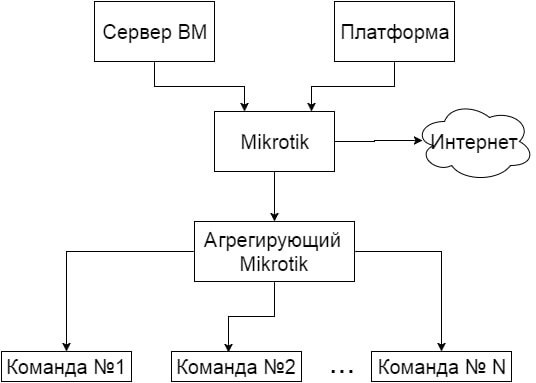
\includegraphics[width=0.8\linewidth]{images/net1.jpg}}
\caption{Схема сети SibirCTF 2015}
\end{figure}
Виртуальная машина каждой команды работала на нашем сервере. У команд были права root. Преимущество данной схемы являлось то, что все команды находились в одинаковых условиях в плане аппартных мощностей.
\newpage

SibirCTF 2016:
На соревнованиях этого года была реализована немного другая схема сети:
\begin{figure}[ht!]
\center{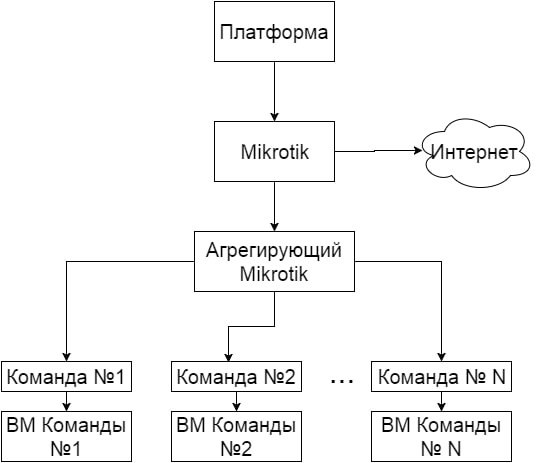
\includegraphics[width=0.8\linewidth]{images/net2.jpg}}
\caption{Схема сети SibirCTF 2016}
\end{figure}

По просьбам участников были предоставлены виртуальные машины. В ходе работы сети были обнаружены следующие проблемы:
\begin{itemize}
\item На момент раздачи образов сеть не справилась с нагрузкой. Это было связано с тем, что пропускная способность канала была ограничена, а образ находился на внешнем ресурсе;
\item В конце соревнований пришлось физически отключить одну команду из-за большого объема трафика, который забивал канал. Также сразу становится виден небольшой недостаток данной схемы сети. Раньше все запросы шли в одно место, на сервер виртуальных машин, теперь маршрутизатор должен был рассылать запросы разным командам. Из-за этого маршрутизатор аппаратно не справлялся с нагрузкой.
\end{itemize}

Выводы, которые были сделаны по итогам соревнований:

\begin{itemize}
\item Образы надо раздавать на флеш-накопителях;
\item Необходимо заменить аппаратный маршрутизатор на программный (по примеру RuCTF, где он себя отлично показал).
\end{itemize}
